\documentclass[../main.tex]{subfiles}
\graphicspath{{\subfix{}}}

\begin{document}

\section{Design}
\label{sec:design}

\subsection{Chosen Components}

\subsubsection{DCS Controller} An Arduino MEGA 2560 Rev3 was chosen as the DCS for this project. Initially we intended on using an Arduino Uno Rev3 however the device did not contain enough memory for us to provide it with the generated code (by 4\%).

\subsubsection{SCADA Supervisor} A Raspberry Pi v4 is being used as the SCADA controller, however a significant portion of testing was done using a Framework 16 Latop.

\subsubsection{Tubing} Quarter inch thick, clear plastic tubing is used for all actuator connections where liquid is transported.

\subsubsection{Container/Project Platform} A three compartment plastic divider is being used as the platform for this project. The middle compartment was removed and is being used as space to place the valves and flowrate sensors. Holes were placed in the bottom of the top container (the container that is being level controlled) with fittings added for hose connections.

\subsubsection{Pumps} HiLetgo DC 12V water pumps were used to move water up (into the controlled vessel) and down (out of the controlled vessel).

\subsubsection{Valves} 12V normally closed solenoid valves were used to stop siphoning when pumping water down, and to implement a manually controlled valve that allows water to be emptied from the upper container.

\subsubsection{Water-Level Sensor} A ruler-style analog water level sensor is used to determine the water level of the container. This is the primary input for determining actuation.

\subsubsection{Temperature Sensor} It was suggested that temperature would be a good metric to track inside our system, however due to scope reduction it was not implemented.

\subsubsection{Flowrate Sensor} It was suggested that flowrate detection across our pumps would be a good metric to track inside our system allowing PID style control with feedback, however due to scope reduction it was not implemented.

\subsection{Electronics}
An Arduino is not typically capable of delivering sufficient current to actuation devices such as pumps and solenoids. To alleviate this issue, a 12V DC supply is used to power the Arduino (barrel connection) and a set of relays. These relays are what is used to drive the pumps and valves, the Arduino simply outputs (digital) to these devices at 5V. The Raspberry Pi is separately powered. The wiring was connected using Wago connectors, and utilized wires of various gauges.

\subsection{Manual Switches}
Several manual switches are present that allow a single valve to be manually controlled, and system power to be manually controlled. This is implemented using simple rocker-style switches.

\subsection{Network}
To isolate our network (for SSH and GUI connection purposes), a TP-Link nano-router was used as a network extender for my Laptop's hotspot. This allows any device connected to that hotspot to wirelessly command the SCADA system.




% Ragged-right paragraph column (avoids hyphenation pressure)
\newcolumntype{P}[1]{>{\raggedright\arraybackslash}p{#1}}
 
% Header style: bold, top-left, no extra gap
\renewcommand\theadfont{\bfseries\small}
\renewcommand\theadgape{}

% ==============================================================
% TABLE I — Sensors
% ==============================================================
\begin{table*}[p]
  \centering
  \footnotesize
  \renewcommand{\arraystretch}{1.4}
  \setlength{\tabcolsep}{5pt}
  \caption{Sensors chosen for the control system.}
  \label{tab:sensors}
  \begin{tabular}{|P{1.8cm}|P{2.6cm}|P{5.8cm}|P{5.8cm}|}
    \hline
    \makecell[tl]{Sensor}
      & \makecell[tl]{Item Name}
      & \makecell[tl]{Role}
      & \makecell[tl]{Implementation Details} \\
    \hline
    Water Level Sensor
      & \textbf{Robot Contact Water/Liquid Level Sensor}
      & Detects if water in the tank reaches a high or low point.
        Prevents overfilling or running dry.
      & Optical sensor output (HIGH/LOW). Connect to GPIO input.
        Can trigger pump ON/OFF automatically. \\
    \hline
    Flow Rate Sensor
      & \textbf{1/4'' Water Flow Sensor (Hall-Effect)}
      & Measures water flow rate in L/min to ensure the pump is
        moving water and to calculate total volume.
      & Generates digital pulses proportional to flow.
        Connect to GPIO input; count pulses using interrupt. \\
    \hline
    Temperature Sensor
      & \textbf{NTC Thermistor 10\,k$\Omega$ MF52-103}
      & Measures the water temperature.
        Can detect overheating or environmental changes.
      & Analog sensor. Use an ADC module (e.g.\ MCP3008) to read
        voltage, then convert to temperature in code. \\
    \hline
  \end{tabular}
\end{table*}
 
 
% ==============================================================
% TABLE II — Actuators
% ==============================================================
\begin{table*}[p]
  \centering
  \footnotesize
  \renewcommand{\arraystretch}{1.4}
  \setlength{\tabcolsep}{5pt}
  \caption{Actuators used in the control system.}
  \label{tab:actuators}
  \begin{tabular}{|P{1.8cm}|P{3.2cm}|P{5.2cm}|P{5.8cm}|}
    \hline
    \makecell[tl]{Actuator}
      & \makecell[tl]{Item Name}
      & \makecell[tl]{Role}
      & \makecell[tl]{Implementation Details} \\
    \hline
    Water Pump
      & \textbf{HiLetgo DC 12\,V 240\,L/h Micro Brushless Pump}
      & Pumps water into or out of the tank.
        Controlled automatically based on level sensor input.
      & Connect through the Pump Controller (relay/MOSFET)
        that switches the 12\,V power. \\
    \hline
    Hydraulic Valve
      & \textbf{1/4'' DC 12\,V 2-Way Normally Closed Solenoid
               Valve (WIC Valve 2ACK Series)}
      & Opens/closes to allow or stop water flow.
      & Controlled through the Valve Controller.
        When the coil is energized, the valve opens;
        otherwise, it closes. \\
    \hline
  \end{tabular}
\end{table*}
 
 
% ==============================================================
% TABLE III — Controllers
% ==============================================================
\begin{table*}[p]
  \centering
  \footnotesize
  \renewcommand{\arraystretch}{1.4}
  \setlength{\tabcolsep}{5pt}
  \caption{Modules interfacing the Raspberry Pi with actuators.}
  \label{tab:controllers}
  \begin{tabular}{|P{2cm}|P{2.2cm}|P{5.8cm}|P{5.8cm}|}
    \hline
    \makecell[tl]{Controller}
      & \makecell[tl]{Connected To}
      & \makecell[tl]{Role}
      & \makecell[tl]{Implementation} \\
    \hline
    Pump Controller
      & Water Pump
      & Acts as a switch driver---receives a 3.3\,V signal from
        the Pi to toggle 12\,V power to the pump.
      & Can be a relay board or a MOSFET circuit.
        Isolates the Pi from the high-power pump. \\
    \hline
    Valve Controller
      & Hydraulic Valve
      & Same principle as the Pump Controller, but for
        opening/closing the valve.
      & When Pi output is HIGH $\rightarrow$ coil energized
        $\rightarrow$ valve opens.
        When LOW $\rightarrow$ valve closes. \\
    \hline
  \end{tabular}
\end{table*}
 
 
% ==============================================================
% TABLE IV — SCADA / HMI
% ==============================================================
\begin{table*}[p]
  \centering
  \footnotesize
  \renewcommand{\arraystretch}{1.4}
  \setlength{\tabcolsep}{5pt}
  \caption{SCADA / Human--Machine Interface components.}
  \label{tab:scada}
  \begin{tabular}{|P{2.4cm}|P{2.4cm}|P{11cm}|}
    \hline
    \makecell[tl]{Component}
      & \makecell[tl]{Role}
      & \makecell[tl]{Description} \\
    \hline
    Laptop / Computer
      & CLI or GUI
      & Acts as the human--machine interface (HMI) for remote
        monitoring and manual control. \\
    \hline
    Wireless Communication
      & Local Area Wifi
      & Connects the Raspberry Pi to the laptop using Wi-Fi.
        Can send real-time data or receive control commands. \\
    \hline
    Software Options
      & Data Visualization
      & \textbf{Flask Web Server:} Allows CLI or GUI to send commands to SCADA.
        \textbf{Plotly:} Allows GUI to poll SQL database to generate plots.
        \textbf{SSH:} Remote access for starting and troubleshooting server.\\
    \hline
  \end{tabular}
\end{table*}
 
 
% ==============================================================
% TABLE V — Communication Links (Pi--Arduino)
% ==============================================================
\begin{table*}[p]
  \centering
  \footnotesize
  \renewcommand{\arraystretch}{1.4}
  \setlength{\tabcolsep}{5pt}
  \caption{Communication link options between the Raspberry Pi and Arduino.}
  \label{tab:comms}
  \begin{tabular}{|P{3.2cm}|P{3cm}|P{3cm}|P{6.6cm}|}
    \hline
    \makecell[tl]{Link}
      & \makecell[tl]{Pros}
      & \makecell[tl]{Cons}
      & \makecell[tl]{Method} \\
    \hline
    \textbf{USB Serial (UART over USB)}
    \textit{(Recommended)}
      & Easiest; powered and isolated via cable; stable.
      & Requires a USB cable.
      & Connect Arduino to Pi via USB; use
        \texttt{/dev/ttyACM0} or \texttt{/dev/ttyUSB0}
        at 115200\,baud. \\
    \hline
    \textbf{I$^{2}$C} (Pi master, Arduino slave)
      & Simple 2-wire interface.
      & 3.3$\leftrightarrow$5\,V level shifting; address management.
      & Pi SDA/SCL $\leftrightarrow$ Arduino A4/A5 (Uno);
        add bi-directional level shifter. \\
    \hline
    \textbf{SPI}
      & Fast throughput.
      & Chip-select management; level shifting required.
      & Pi SPI0 $\leftrightarrow$ Arduino SPI pins;
        level shifter required. \\
    \hline
    \textbf{RS-485 (Modbus RTU)}
      & Long cable runs; noise-robust.
      & Requires transceivers and protocol stack.
      & MAX485 modules, twisted-pair cable, Modbus library. \\
    \hline
  \end{tabular}
\end{table*}
\clearpage

\begin{figure*}[p]
    \centering % Centers the image
    \rotatebox{90}{
    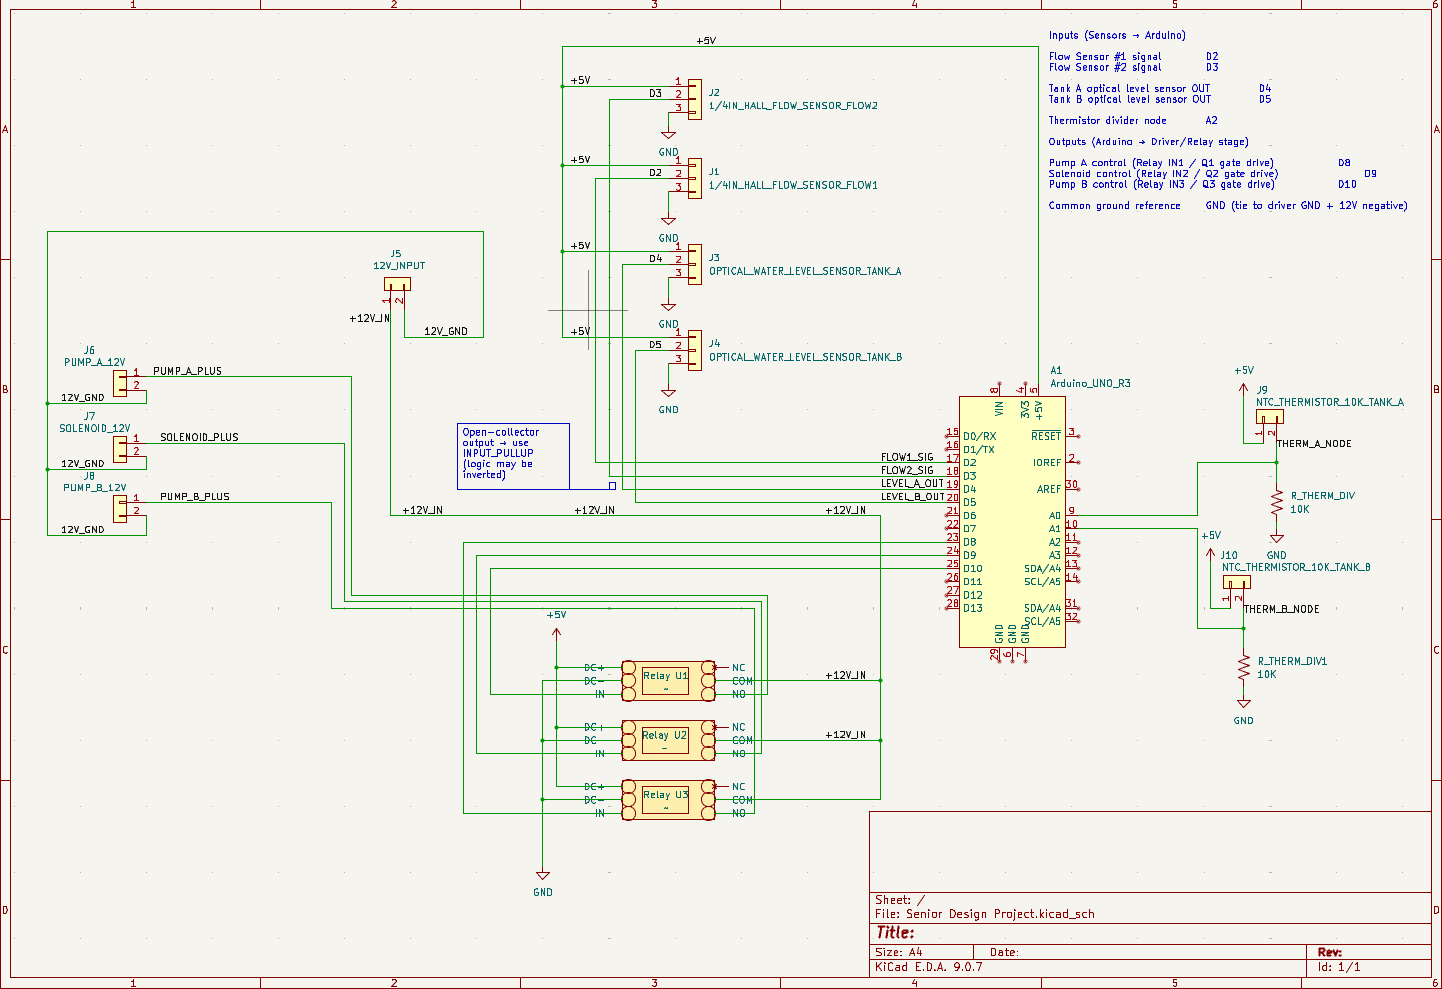
\includegraphics[width=1.25\textwidth]{../fig/Initial_Schem}} % Image file without extension
    \caption{Initial Hardware Schematic}
    \label{fig:Initial_Schem} % Used for \ref{fig:my_label} in text
\end{figure*}
\clearpage

\begin{figure*}[p]
    \centering % Centers the image
    \rotatebox{90}{
    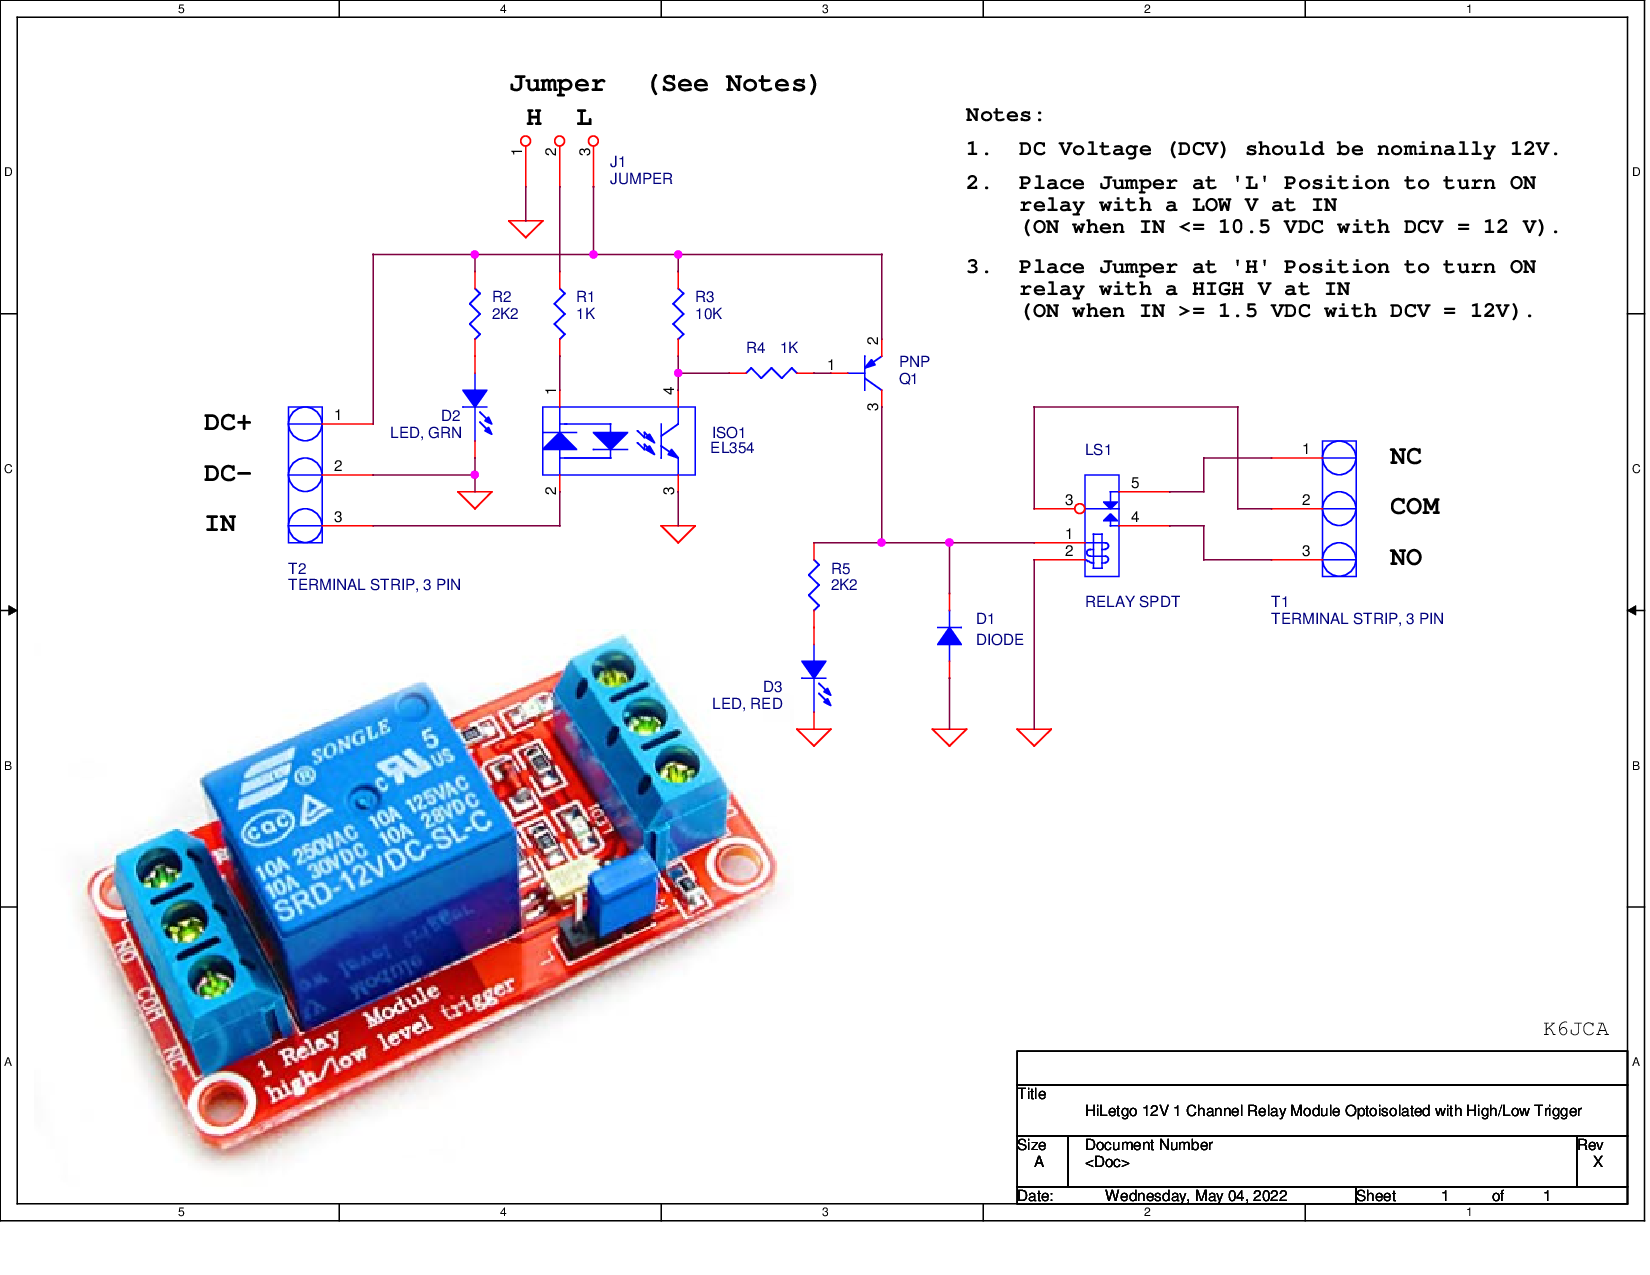
\includegraphics[width=1.25\textwidth]{../fig/Final_Schem}} % Image file without extension
    \caption{Final Hardware Schematic}
    \label{fig:Final_Schem} % Used for \ref{fig:my_label} in text
\end{figure*}
\clearpage

\subsection{Software Design}
The design of the SCADA software was done in piece-wise as new features were added, however the code-base utilizes multithreading to ensure all asynchronous operations are non-blocking to the main thread. The code-base is comprised of the following major sections.

\subsubsection{Main Thread} The main thread (and entry point) is the contained in the executable SCADA.py. When this is initialized it will ensure a data path (outside of the repository path) is established for data and settings to be stored inside of on the host system. It will then initialize all other needed threads and facilitate pass-by-reference communication with and between all other threads.

\subsubsection{Serial Thread} The serial (monitor) thread is the first thread to launch, it continuously monitors the host system's serial ports, updating the main thread when connection or disconnection events occur. This allows the main thread to run a set of functions for each event to determine whether the detection is an Arduino or if it should be ignored.

\subsubsection{Flask Thread} The Flask thread launches a Flask backend-server that accepts POST commands (and filters inputs for invalid requests), this is the entry point to the software, both the CLI and the GUI simply access exposed commands in the Flask thread and it facilitates the rest of the SCADA-side logic. This thread also opens port 5000 for CLI and GUI connections.

\subsubsection{Worker Thread(s)} When a serial connection event is detected in the main thread, and this connection happens to be an Arduino, a worker thread is created for the Arduino' port. This thread both sends hold commands requested (via the Flask thread) and collects data at a user-specified polling rate and stores it in the SQL database (in the created data-path). This thread terminates itself when the Arduino is disconnected.

\subsubsection{Controller Initialization} When a controller is connected for the first time, a JSON file containing all port configurations, user defined code blocks and settings is saved with default settings into the data path in a folder called ``dcs\_info". This and all settings modifications are defined in a python file called dcs\_dict\_utils which is by far the longest back-end file in this project. The functions in this section determine rules for pin and point interactions and settings, as well as the use of arrays, timers, ISRs and more. The combination(s) of settings achievable is detailed enough for code-generation, but there would be no implemented logic.

\subsubsection{Code Blocks} Code blocks are semi-generically typed blocks that can be placed into any region in the controller's code, such as setup, loop, and inside of any ISR. The available ISRs are kept in a list (via many functions working in tandem within dcs\_dict\_utils) and update based on pin-driven interrupt settings and timer settings. Code blocks, such as the addition block, have some inputs (the two input numbers in this case), sometimes a number of outputs (in this case the sum), and a slot for a boolean variable that is used as a conditional statement. Some code blocks require an array as an input or output and cannot accept a point.

\subsubsection{Points} Points as defined in the code-base are essentially software variables that can represent hardware (such as the points locked to pins or timer registers) or can be user defined (such as a user defined int, float, or bool). Points can be held over serial (via the worker threads) to a user-defined value, and points can be configured with a minimum and maximum. Internally to the Arduino, all points are a 5-value struct, but they are treated as a single variable using getter and setter commands (in generated code).

\subsubsection{Code Validation} Before code can be generated, many simple rules are evaluated to determine whether the user-defined code-script makes sense. For example, a point being the output of two code-blocks causes a conflict, as such the validation will return a string listing that error. When an empty string is returned, the code-generation pipeline can proceed.

\subsubsection{Code Generation} Using the configuration generated from the rules in dcs\_dict\_utils, and using the code-block logic defined in code\_block\_utils, the file ino\_utils can be used to generate (mostly) feature complete Arduino AVR C++ code. All points and arrays get defined at the top and evaluated for whether they need to be constants or volatile based on the user-defined settings saved to file. Then a generic form of each code block (only those used at least once) is defined once in setup. Then in each section code-blocks were placed, a call to that block using the point getter function for each input (except for arrays) is used, and the outputs are assigned via the point setter function. Finally at the end of loop the Arduino is told to print all point values so that the worker thread can log them, and checks if the worker thread wrote a hold command which gets set to the specified point.

\subsubsection{Uploading Code to an Arduino} Once an ino file is generated (which will share the same name as the controller in question), upon command the Flask server can push a queue request for a controller to be flashed by port name, this is passed to the main thread where the main thread passes it to both the worker in question and the flash thread. The worker must close its port before the flash thread can continue, but regains port control once flashing is complete (or fails).

\subsubsection{Command Line Interface}
During development and debugging the CLI was used to interact with the Flask server. Though the CLI is feature complete in terms of usability, it is far less pleasant than the GUI. The GUI was one of the last features added to the code, which meant the CLI received a lot of use. To use the CLI it can be run as a separate python file on the host machine, and when `help' is entered it lists all valid commands.

\subsubsection{Graphical User Interface}
The GUI is a simple web-UI that is launched at localhost:5000 on the host machine, and can be accessed by typing ``http://\{ip\}:5000" into the searchbar of any browser where \{ip\} is the local IP address of the host system, or ``localhost" if launching from the host system. This GUI allows the code-block system to be used as a visual code editor, compiled and uploaded with the push of two buttons, and verified with live-updating and historical plotting for all connected controllers simultaneously.




















\end{document}